\documentclass{article}
\usepackage[utf8]{inputenc}
\usepackage{graphicx, amsmath, amssymb, tikz}
\usepackage{hhline}
\usepackage[table]{xcolor}
\usepackage[most]{tcolorbox}
\usepackage{lipsum}
\usepackage{hyperref}
\graphicspath{ {./images/} }
\usepackage[dvipsnames]{xcolor}

\title{Self-Attention and Transformers}
\author{sumit singh}
\date{\today}

\begin{document}

\maketitle
\begin{abstract}
\noindent
Understanding of Transformer architecture.

\end{abstract}

\hspace{0.5in}
\keywords{Positional Encoding, Rotary Positional Embeddings,Embedding, Positional Embeddings, Context Vectors, Residual Connection, Layer Normalization}
%*********************************************************************************************
\section{Motivation for Transformers}
\begin{tcbraster}[raster columns=2,raster equal height,nobeforeafter,raster column skip=0.5cm]
  \begin{tcolorbox}[title=Challenges with RNNs]
    \begin{itemize}
    \item Gradient vanishing and explosion
    \item Large \# of training steps
    \item Sequential computation/Recurrenece prevents parallel computation
    \item Despite GRUs and LSTMs, RNN still need attention mechanism to deal with long-range dependencies - path length for co-dependent computation between states grows with sequence length
\end{itemize}
  \end{tcolorbox}
  \begin{tcolorbox}[title=Transformer Networks]
    \begin{itemize}
    
    \item No gradient vanishing and explosion
    \item Fewer training steps
    \item No recurrence that facilitate parallel computation
    \item Facilitate Long Range Dependencies
\end{itemize}
  \end{tcolorbox}
\end{tcbraster}
But if attention gives us access to any state, maybe we don't need the RNN?!
%*********************************************************************************************    
\section{Attention Mechanism}
%*********************************************************************************************
%*********************************************************************************************   
\begin{minipage}{0.5\textwidth}
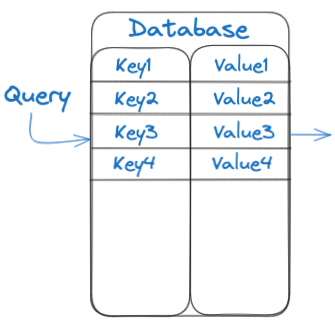
\includegraphics[width=5cm, height=3.5cm]{Transformer/Images/Attention1.png}
\end{minipage}
\begin{minipage}{0.5\textwidth}
\begin{itemize}
    \item Mimics the retrieval of a \textbf{value} $v_i$ for a \textbf{query} $q$ based on a key $k_i$ in database.
    \item $attention(q,\textbf{k},\textbf{v}) = \sum_i similarity(q,k_i)\times v_i$
    \item $s_i = f(q,k_i)$
\end{itemize}
\end{minipage}
%************************************************************************************
%*********************************************************************************************  
\hrule
\textbf{Step 1}: \\
\begin{minipage}{.65\linewidth}
\begin{equation*}
  f(q,k_i)=\begin{cases}
    q^T k_i, & \text{Dot Product}.\\
    \frac{q^T k_i}{\sqrt{d}}, & \text{Scaled Dot Product}.\\
    q^T W k_i, & \text{General Dot Product}. \\
    w_q^T q + W_k^T k_i , & \text{Additive Similarity}
  \end{cases}
\end{equation*}
\end{minipage}
\begin{minipage}{.5\linewidth}
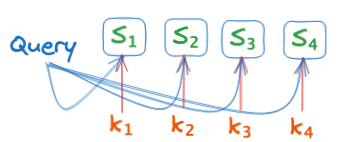
\includegraphics[width=4cm, height=3.5cm]{Transformer/Images/Attention2.png}
\end{minipage}
%************************************************************************************
$s$ corresponds to the similarity measure. $d$ is the dimensionality of each key. $W$: Think of it as if we are transforming our queries to be in the same space as the keys. Kernel methods also measure similarity. They do this by essentially mapping two vectors into a new space through some non-linear function. We could also have here some form of kernel similarity.  \\
\hrule
\textbf{Step 2}:\\
%*********************************************************************************************   
\begin{minipage}{0.5\textwidth}
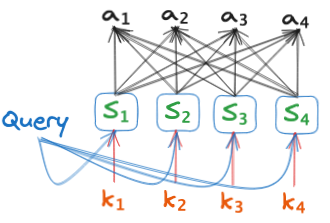
\includegraphics[width=4cm, height=3.5cm]{Transformer/Images/Attention3.png}

\end{minipage}
\begin{minipage}{0.5\textwidth}
\begin{itemize}
    \item The second step/layer is to compute the weights $a_1,a_2,a_3,a_4$.
    \item $a_i = \frac{exp(s_i)}{\sum_j exp(s_j}$. 
    \item This is a fully connected network but not in the classical sense. 
\end{itemize}
\end{minipage}
%************************************************************************************
\hrule 
\textbf{Step 3}:\\
%*********************************************************************************************   
\begin{minipage}{0.5\textwidth}

\begin{itemize}
    \item Attention Value $= \sum_i a_i * v_i$.
    \item $a_i = \frac{exp(s_i)}{\sum_j exp(s_j}$. 
    \item This is a fully connected network but not in the classical sense. 
\end{itemize}
\end{minipage}
\begin{minipage}{0.5\textwidth}
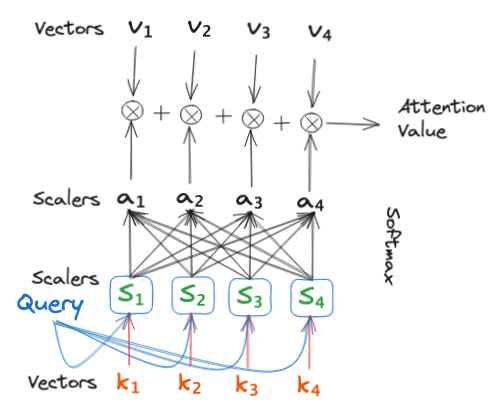
\includegraphics[width=6cm, height=5cm]{Transformer/Images/Attention4.png}
\end{minipage}
%************************************************************************************
\begin{itemize}
    \item Neural Architecture
    \item Example: machine translation
    \begin{itemize}
        \item Query: $s_i$ (hidden vector for $i^{th}$ output word )
        \item Key: $h_j$ (hidden vector for $j^{th}$ input word)
        \item Value: $h_j$ (hidden vector for $j^{th}$ input word)
    \end{itemize}
\end{itemize}
  
%*********************************************************************************************    
\section{Transformer Network}
%*********************************************************************************************   
\begin{minipage}{0.5\textwidth}
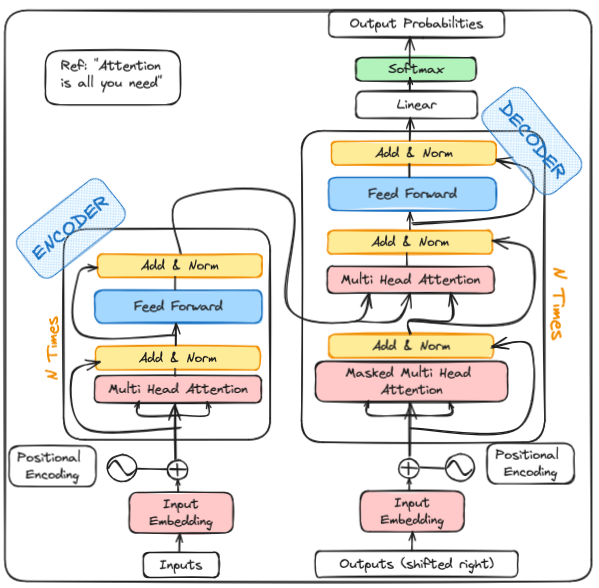
\includegraphics[width=6cm, height=8cm]{Transformer/Images/Transformers1.png}
\end{minipage}
\begin{minipage}{0.5\textwidth}
\begin{itemize}
    \item The work "Attention is All you Need" (Vaswani et al, NeurIPS 2017) first made it possible to do Seq2Seq modelling without RNNs)
    \item Proposed transformer model, entirely built on self-attention mechanism without using sequence-aligned recurrent architectures
    \item Encoder-decoder based on attention (no recurrence)
    \item Key components:
    \begin{itemize}
        \item Self-Attention
        \item Multi-Head Attention
        \item Positional Encoding
        \item Encoder-Decoder Architecture
    \end{itemize}
\end{itemize}
\end{minipage}
Recurrence means that the optimization takes longer for 2 reasons: -
\begin{itemize}
    \item \# of iterations, \# of steps in gradient descent will be higher
    \item We will have several operations that are going to be sequential \& then we cannot parallelize them easily
\end{itemize}
Transformer networks have 2 parts: Encoders and Decoders. In Machine translation, the encoder is used to encode the initial sentence, and the decoder is used to produce the translated sentence. 
%************************************************************************************
\subsubsection{Encoder}
%************************************************************************************
The encoder processes an entire sentence in parallel as opposed to RNN which processes one word at a time in the sentence. Input in TIV is an entire sequence of words which are embedded and then positional encoding is done.
\begin{minipage}{0.6\textwidth}
% Import required TikZ libraries
\documentclass{article}
\usepackage{tikz}
\usetikzlibrary{shapes,shadows, arrows, positioning, fit, backgrounds}
% \begin{document}



% Define block styles
\tikzstyle{decision} = [diamond, draw, fill=yellow!40, 
    text width=4.5em, text badly centered, node distance=1.75cm, inner sep=0pt]
\tikzstyle{decisiong} = [diamond, draw, fill=blue!40, 
    text width=4.5em, text badly centered, node distance=1.75cm, inner sep=0pt]
\tikzstyle{block} = [rectangle, node distance=1.75cm, minimum width=1cm, minimum height=0.5cm, draw, fill=yellow!10, 
    text width=20em, text centered, rounded corners, minimum height=1.5em]
\tikzstyle{blockg} = [rectangle, minimum width=0.5cm, minimum height=0.5cm, draw, fill=blue!10, 
    text width=15em, text centered, rounded corners, minimum height=1.5em]
\tikzstyle{blockh} = [rectangle, minimum width=0.5cm, minimum height=0.5cm, draw, fill=green!10, 
    text width=15em, text centered, rounded corners, minimum height=1.5em]
\tikzstyle{blockwhite} = [rectangle, minimum width=0.5cm, minimum height=0.5cm, draw, fill=white!50, 
    text width=15em, text centered, rounded corners, minimum height=1.5em]
\tikzstyle{line} = [draw, -latex']
\tikzstyle{cloud} = [draw, ellipse,fill=yellow!20, node distance=1.5cm, 
    minimum height=1em]
\tikzstyle{invis} = [draw, fill=yellow!10, node distance=4.25cm, 
    minimum height=2em]
\tikzstyle{invisg} = [draw, fill=yellow!10, node distance=3.5cm, 
    minimum height=2em]
\tikzstyle{matheq} = [node distance=8.75cm, text width=21em, minimum width=1cm, 
    minimum height=2em, text centered]
% Add your preamble here


\begin{tikzpicture}[node distance = 1.25cm, auto]
    % Place nodes
    \node [cloud] (exit) {};

    \node [blockh, below of=exit] (ln1) {Add \& Norm};
    \node [blockg, below of=ln1] (ff) {\textbf{Feed-forward}};
    \node [cloud, below of=ff] (mid) {};
    \node [blockh, below of=mid] (ln2) {Add \& Norm};
    
    \node [blockg, below of=ln2] (sa) {\textbf{Multi-head Attention} };
    \node [cloud, below of=sa] (init) {};
    \node [blockwhite, below of=init] (input) {Encoder };

 

    \begin{scope}[on background layer]
    \node[draw, fill=blue!0, fit=(sa) (ln1), inner xsep=5mm]{};
    \end{scope}
    % Draw edges
    \path [line] (ln1) -- (exit);
    \path [line] (ff) -- (ln1);
    \path [line] (mid) -- (ff);
    \path [line] (ln2) -- (mid);
    \path [line] (sa) -- (ln2);
    \path [line] (init) -- (sa);

    \path [line] (init) -| ([xshift=3cm, yshift=0cm]init.east) |- (ln2);
    \path [line] (mid) -| ([xshift=3cm, yshift=0cm]mid.east) |- (ln1);


% https://tex.stackexchange.com/questions/142548/tikz-complicated-flow-chart

\end{tikzpicture}

% \end{document}
\end{minipage}
\begin{minipage}{0.5\textwidth}
The important part of the transformer network is the encoder block. It consists of two sub-parts:
\begin{itemize}
    \item Multi-head Attention
    \item Feed Forward Neural Network
\end{itemize}
\end{minipage}
The Multi Head Attention is where all the good stuff happens. A vector which consists of sub-vectors of all the words that we have in our sentence is fed in.  Then the \textit{Multi Head Attention} is going to compute the attention between every position and every other position. A vector which consists of sub-vectors of all the words we have in our sentence is fed in. Then the Multi Head Attention is going to compute the attention between every position and every other position. \\
We have vectors that embed the word in each of those positions \& now we simply \textit{\textcolor{red}{carry out an attention computation that will essentially treat each word as a query then find some keys that corresponds to the other words in the sentence \& then take a convex combination of the corresponding values. Here the values are going to be the same as the keys \& then take a distribution of that to produce a better embeddings.}} \\
The Multi-Head-Attention will essentially take every word, combine it with some of the other words through the attention mechanism to essentially produce better embeddings that merge together information from pairs of words. When we do this in one encoder block, we essentially look at pairs of words together. We repeat the encoder block $N$ times ($N$ stacks). In the first block, we are looking at pairs. In the second block, we are looking at pairs of pairs.  We are now combining more than just two words: groups of words that get larger and larger. \\
Then we  have another layer \textit{Add \& Norm}. This adds the original input and the output from Multi Head Attention. Then it normalizes it with zero mean and unit variance.\\
This output is fed into a \textit{feed forward} network whose output, along with residual connection addition, is finally normalized.\\
The above is the encoder block which is repeated $N$ times. This means we not only combine pairs of words but also pairs of pairs of words and so on. Eventually, we combine together all the words in the sentence. \\
The output of the encoder block is a sequence of embeddings. There is going to be one embedding per position. The embedding captures not only the original word at this position but also information from the other words that it attended to throughout the network. Eventually, it is a large embedding of all those words corresponding to each position. This is our final encoding of the input sentence. \\

%************************************************************************************
\subsubsection{Decoder}
%************************************************************************************
The Decoder follows the encoder and does something similar. The main purpose of the decoder is to produce some output and not just embed. So we have additional stuff at the top - softmax. Softmax outputs the probabilities for outputting a label in each position. The decoder block also repeats $N$ times. \\
Inside the decoder block we have first a Multi Head Attention that looks at combining output words with previous output words. There is a second block of Multi Head Attention that now combines output words with input words. Finally, a feed forward network.  Hence, we have two layers of attention in the decoder.  The first layer is for self attention between the output words. The problem with output words is when you generate a sequence of output you can only generate the next words based on previous words. So, when you do the attention you need to be careful to attend only to the previous words. This is why it is called a \textit{Masked Multi Head Attention}. The future word is masked, each word is only attending to the previous words. The second Multi Head Attention in the decoder is making sure that each position in the output is attending to the positions in the input. Whenever you produce an output it's good if you can peek and look back at what was your input sentence. Hence we are going to look at the embeddings of each position in the input and hence the arrows from the encoder to the decoder. The Decoder is also repeated $N$ times. The idea is we gradually built up combinations and then get better and better embeddings unless we produce an output. \\
The output is a distribution over the words in a dictionary. Every position is a word that we are trying to generate.
%************************************************************************************
\subsubsection{Transformers in a Nutshell}
\begin{minipage}{0.5\textwidth}
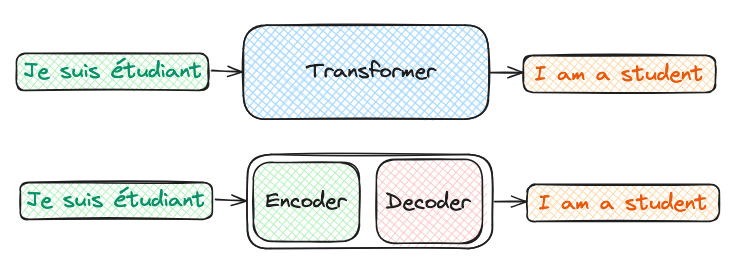
\includegraphics[width=6cm, height=3cm]{Transformer/Images/Transformers2.png}
\end{minipage}
\begin{minipage}{0.5\textwidth}
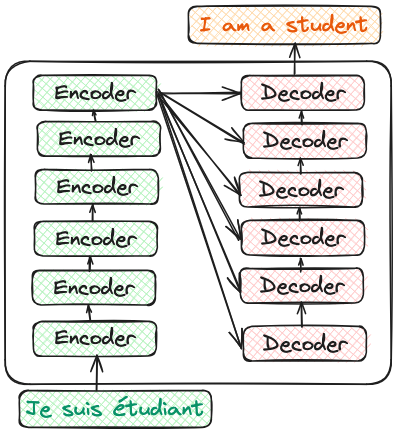
\includegraphics[width=6cm, height=5cm]{Transformer/Images/Transformers3.png}
\end{minipage}
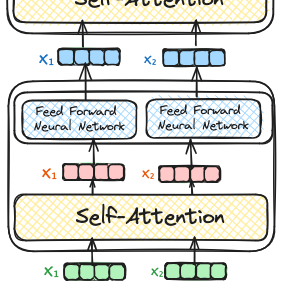
\includegraphics[width=6cm, height=6cm]{Transformer/Images/Transformers4.png}
%************************************************************************************
%************************************************************************************
\section{Self-Attention}
%************************************************************************************
\begin{itemize}
    \item Consider two input sentences we want to translate:
    \begin{itemize}
        \item The \textcolor{red}{animal} didn't cross the street because it was too \textcolor{red}{tired}
        \item The animal did not cross the  \textcolor{red}{street} because it was too \textcolor{red}{wide}
    \end{itemize}
    \item "it" refers to "animal" in the first case, but to "street" in the second case
    \item This is hard for traditional \textit{Seq2Seq} models to model.
    \item As the model processes each word, self-attention allows it to look at other positions in the input sequence to help get a better encoding. 
    \item Recall RNNs: we now no longer need to maintain a hidden state to incorporate the representation of previous words/vectors!
\end{itemize}
%************************************************************************************
\subsection{Self-Attention: keys, queries, values from the same sequence}
Let $\textbf{w}_{1:n}$ be a sequence of words in vocabulary $V$, like \textit{I am a cartoon}. For each $\textbf{w}_i$ , let $\textbf{x}_i = E w_i$ , where $E \in \mathbb{R}^{d \times |V|}$ is an embedding matrix.  \\

\begin{itemize}
    \item Transform each word embedding with weight matrices $Q,K,V$, each in $\mathbb{R}^{d \times d}$
        \begin{align*}
            q_i &= Q x_i &\qquad & \text{(queries)} \\
            k_i &= K x_i && \text{(keys)} \\
            v_i &= V x_i && \text{(values)} 
        \end{align*}
    \item Compute pairwise similarities between keys and queries; normalize with softmax
        \begin{align*}
            e_{ij} &= q_i^T k_j \\
            \alpha_{ij} &= \frac{exp(e_{ij})}{\sum_{j'} exp(e_{ij'})}
        \end{align*}
    \item Compute output for each word as weighted sum of values
        \begin{align*}
            o_i = \sum_j \alpha_{ij} v_i 
        \end{align*}
\end{itemize}
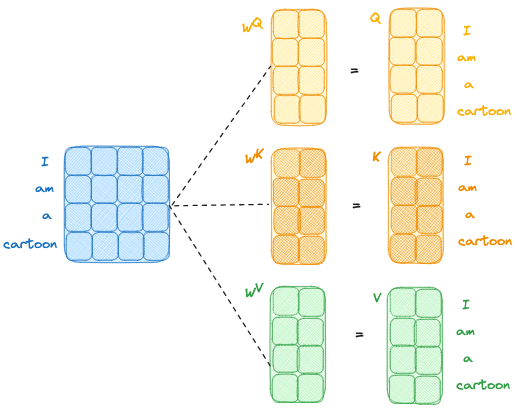
\includegraphics[width=6cm, height=6cm]{Transformer/Images/Attention5.png} \\
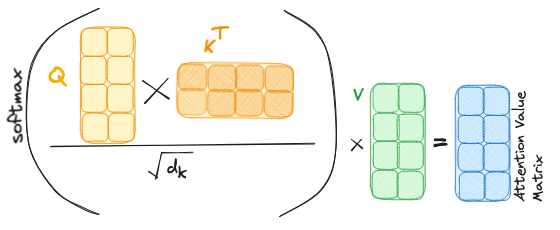
\includegraphics[width=10cm, height=6cm]{Transformer/Images/Attention6.png}
\begin{align*}
    
\end{align*}

\subsection{Next}
%************************************************************************************
\begin{minipage}{0.5\textwidth}
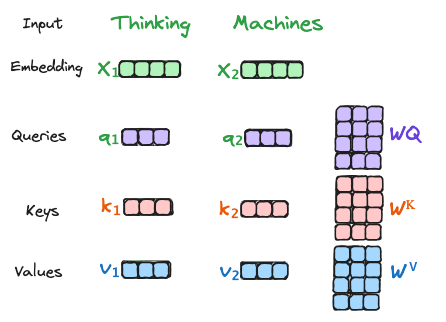
\includegraphics[width=6cm, height=6cm]{Transformer/Images/SelfAttention1.png}
\end{minipage}
\begin{minipage}{0.5\textwidth}
\begin{itemize}
    \item \textbf{STEP 1}: Create three vectors from encoder's input vector ($x_i$):
    \begin{itemize}
        \item Query vector ($q_i$)
        \item Key vector ($k_i$)
        \item Value vector ($v_i$)
    \end{itemize}
    \item These are created by multiplying input with weight matrices $W^Q, W^K, W^V$, learned during training.
    \item In the paper $q,k,v \in \mathbb{R}^{64} $ and $x \in \mathbb{R}^{512}$
    \item Do $q,k,v$ always have to be smaller than $x$? No, this was done perhaps to make computation of multi-headed attention constant
    \item What are the dimensions of $W^Q, W^K, W^V$?
\end{itemize}
\end{minipage}
\\
%************************************************************************************
\begin{minipage}{0.5\textwidth}

\begin{itemize}
    \item \textbf{STEP 2}: Calculate self-attention scores - Score all words of input sequence against themselves. How?
    \item By taking dot product of \textcolor{blue}{query vector} with \textcolor{blue}{key vector} of respective words
    \item E.g. for input "Thinking", first score would be $q_1 \cdot k_1 $
    \item  (with itself); second score would be dot product of $q_1 \cdot k_2$ (with "Machines"), and so on.
    \item Scores then divided by $\sqrt{length(k)}$
    \item This is \textcolor{blue}{Scaled Dot-Product Attention},. This design choice leads to more stable gradients.
\end{itemize}
\end{minipage}
\begin{minipage}{0.5\textwidth}
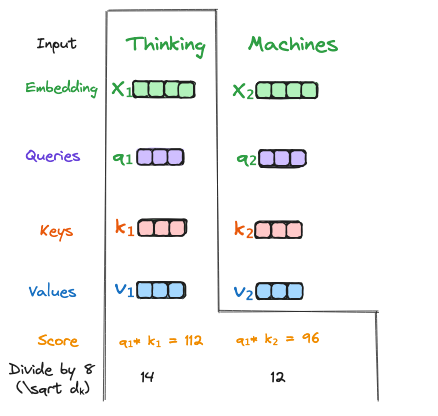
\includegraphics[width=6cm, height=6cm]{Transformer/Images/SelfAttention2.png}
\end{minipage}
%************************************************************************************
\begin{minipage}{0.5\textwidth}
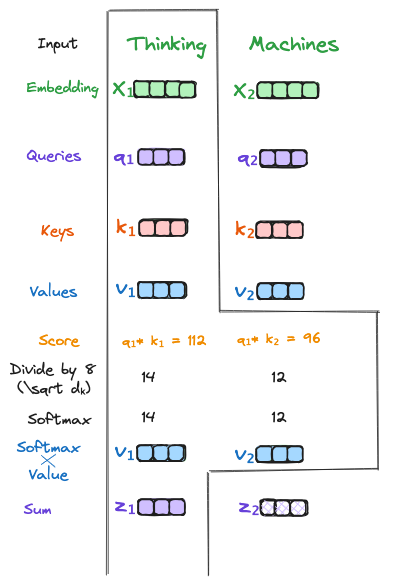
\includegraphics[width=6cm, height=8cm]{Transformer/Images/SelfAttention3.png}
\end{minipage}
\begin{minipage}{0.5\textwidth}
\begin{itemize}
    \item \textbf{STEP 3}: Softmax used to get normalized probability scores; determine how much each word will be expressed at this position
    \item Clearly, word at this position will have highest softmax score, but sometimes it's useful to attend to another word that is relevant
    \item \textbf{STEP 4}: Multiply each \textcolor{blue}{value vector} by softmax score. Why? Keep value of word(s) we want to focus on intact, and drawn out irrelevant words
    \item \textbf{STEP 5}: Sum up weighted value vectors $\rightarrow$  produces output of self-attention layer at this position (for first word)
\end{itemize}
\end{minipage}
%************************************************************************************
\begin{minipage}{0.5\textwidth}
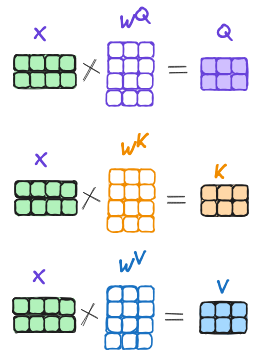
\includegraphics[width=6cm, height=5cm]{Transformer/Images/SelfAttention4.png}
\end{minipage}
\begin{minipage}{0.5\textwidth}
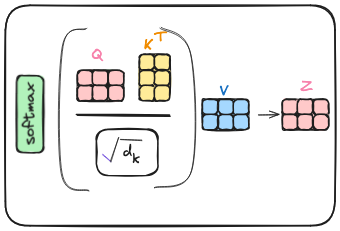
\includegraphics[width=6cm, height=5cm]{Transformer/Images/SelfAttention5.png}
\end{minipage}

For each attention head \textbf{we need a query, key and value vector for each input token}. We then compute \textbf{attention score} as the softmax over the \textbf{scaled dot product} between one query and all key vectors in the sentence. The equation below computes an \textbf{  attention-weighted } average over all value vectors for each input token at once. \textbf{Q} is the matrix that stacks \textbf{q}uery vectors for all input tokens: \textbf{K} and \textbf{V} do the same for \textbf{k}ey and \textbf{v}alue vectors.
\begin{equation}
    Attention(Q,K,V) = softmax (\frac{QK^T}{\sqrt{d_k}})V
\end{equation}
%************************************************************************************
%************************************************************************************
\section{Multi-Head Attention}
%************************************************************************************
%************************************************************************************
\begin{itemize}
    \item Multihead attention: compute multiple attentions per query with different weights
    \item $multihead(Q,K,V) = W^0 concat(head_1, head_2, \cdot , head_h)$ 
    \item $ head_i = attention(W_i^QQ, W_i^K K, W_i^V V )$
    \item $attention(Q,K,V) = softmax(\frac{Q^T K}{\sqrt{d_k}} )V$ 
\end{itemize}



%************************************************************************************
\begin{minipage}{0.5\textwidth}
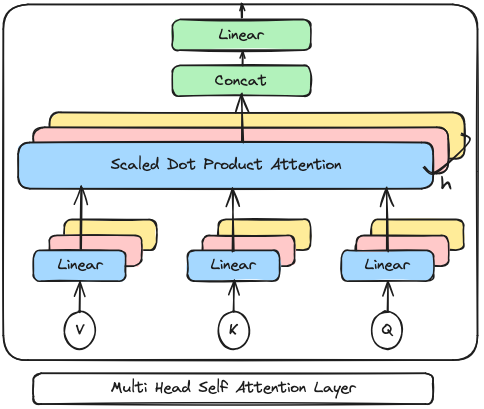
\includegraphics[width=6cm, height=8cm]{Transformer/Images/MultiHeadAttention1.png}
\end{minipage}
\begin{minipage}{0.5\textwidth}
\begin{itemize}
    \item Improves performance of the attention layer in two ways:
    \begin{itemize}
        \item Expands model's ability to focus on different positions. In example above, $z_1$ contains a bit of every other encoding, but dominated by actual word itself.
        \item Gives attention layer multiple "representation subspaces"; we have not one but multiple sets of Query/Key?value weight matrices; after training, each set is used to project input embeddings into different representation subspaces
    \end{itemize}
    \item $h \rightarrow $ \# of head 
\end{itemize}
\end{minipage}
%************************************************************************************
\begin{minipage}{0.5\textwidth}
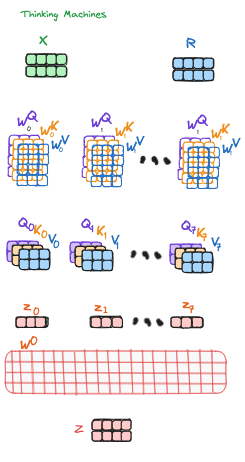
\includegraphics[width=6cm, height=10cm]{Transformer/Images/MultiHeadAttention2.png}
\end{minipage}
\begin{minipage}{0.5\textwidth}
\begin{itemize}
    \item This is our input sequence *
    \item We embed each word * \\
    \item Split into 8 heads. We multiply \textcolor{green}{X} or \textcolor{blue}{R} with weight matrices.
    \item Calculate attention using the resulting \textcolor{pink}{Q}/ \textcolor{orange}{K}/ \textcolor{blue}{V} matrices
    \item Concatenate the resulting \textcolor{pink}{Z} matrices, then multiply with weight matrix \textcolor{pink}{$W^0$} to produce the output of the layer
\end{itemize}
\end{minipage}
$\ast$ In all encoders other than 0, we don't need embedding. We start directly with the output of the encoder right below this one.
%************************************************************************************
\subsection{Masked Multi-head Attention}
\begin{itemize}
    \item Masked multi-head attention: multi-head where some values are masked (i.e., probabilities of masked values are nullified to prevent them from being selected)
    \item When decoding, an output value should only depend on previous outputs (not future outputs). Hence we mask future outputs.
    \item $attention(Q,K,V) = softmax(\frac{Q^T K}{\sqrt{d_k}})V$
    \item $maskedAttention(Q,K,V) = softmax(\frac{Q^T K + M}{\sqrt{d_k}})$
    \item where $M$ is a mask matrix of $0$'s and $-\infty$'s
\end{itemize}
%************************************************************************************
\subsection{Other Layers}
\begin{itemize}
    \item Layer Normalization
    \begin{itemize}
        \item Normalize value in each layer to have $0$ mean and $1$ variance
        \item For each hidden unit $h_i$ compute $h_i \leftarrow  \frac{g}{\sigma} (h_i - \mu)$ where $g$ is a variable, $\mu = \frac{1}{H} \sum_{i=1}^H h_i$ and $\sigma = \sqrt{\frac{1}{H} \sum_{i=1}^H (h_i - \mu)^2 }$
        \item This reduces "covariate shift" (i.e., gradient dependencies between each layer) and therefore fewer training iterations are needed
    \end{itemize}
    \item Positional Embeddings
\end{itemize}
%************************************************************************************
%************************************************************************************
\section{Positional Encoding}
%************************************************************************************
%************************************************************************************
\begin{itemize}
    \item Embedding to distinguish each position
    \item Unlike RNN and CNN encoders, attention encoder outputs do not depend on order of inputs (Why?)
    \item But order of sequence conveys important information for machine translation tasks and language modeling
    \item The idea: Add positional information of input token in the sequence into input embedding vectors
\end{itemize}
\begin{align*}
    &PE_{pos,2i}   &= sin \frac{pos}{1000^{\frac{2i}{d_{emb}}}} \\
    &PE_{pos,2i+1} &= cos \frac{pos}{1000^{\frac{2i}{d_{emb}}}}
\end{align*}
\begin{itemize}
    \item Final input embeddings are concatenation of learnable embedding and positional encoding
    \item position is scalar. Position embedding is vector.
\end{itemize}
%************************************************************************************
%************************************************************************************
\section{Conclusion}
%************************************************************************************
%************************************************************************************
\begin{itemize}
    \item Attention reduces sequential operations and maximum path length, which facilitates long range dependencies
\end{itemize}
\begin{tabular}{ |p{4cm}||p{2cm}|p{2cm}|p{3cm}|  }
 \hline
 \multicolumn{4}{|c|}{Comparison} \\
 \hline
 Layer Type& Complexity per Layer &Sequential Operations & Maximum Path Length\\
 \hline
 Self-Attention   & $O(n^2 \cdot d)$     & $ O(1) $ &   $ O(1) $\\
 Recurrent &   $O(n \cdot d^2)$  & $ O(n) $   & $ O(n) $\\
 Convolutional & $O(k \cdot n \cdot d^2)$  & $ O(1) $ &  $ O( log_k(n) ) $\\
 Self-Attention(restricted)    & $O(r \cdot n \cdot d^2)$  & $ O(1) $ &   $ O(n/r) $\\
 \hline
\end{tabular}

%************************************************************************************
%************************************************************************************
\section{References}
%************************************************************************************
\begin{itemize}
    \item \href{https://www.youtube.com/watch?v=phOc25QfNS0&t=55s}{NPTEL Lecture}
    \item \href{https://courses.cs.washington.edu/courses/cse543/22sp/schedule/lecture15_transformer.pdf}{CS Washington}
    \item \href{https://www.youtube.com/watch?v=5V9gZcAd6cE}{Positional encodings in transformers (NLP817 11.5)}
    \item \href{https://www.cs.ubc.ca/~schmidtm/Courses/440-W22/L20.pdf}{CPSC 440}
    \item \href{https://www.cs.toronto.edu/~rgrosse/courses/csc421_2019/slides/lec16.pdf}{CS Toronto CSC 421}
    \item \href{https://web.stanford.edu/class/cs224n/slides_w25/cs224n-2025-lecture08-transformers.pdf}{Stanford CS 224n}
    \item \href{https://jorisbaan.nl/2022/03/25/implementing-a-transformer-from-scratch.html}{Joris Baan}
\end{itemize}
\end{document}